% Latex template: mahmoud.s.fahmy@students.kasralainy.edu.eg
% For more details: https://www.sharelatex.com/learn/Beamer

\documentclass{beamer}					% Document class

\usepackage[english]{babel}				% Set language
\usepackage[utf8]{inputenc}			% Set encoding

% \usetheme{metropolis} % Preferred beamer theme

\usepackage{graphicx} % Load graphics
\usepackage{booktabs} % Nice tables
\usepackage{dcolumn} % Booktabs column spacing
\usepackage{threeparttable} % Align column caption, table, and notes
\usepackage{adjustbox} % Shrink stuff
% \usepackage{showframe} % Useful for debugging
\usepackage{amsthm}
\usepackage{amsmath}
\usepackage{amsfonts}
\setbeamertemplate{theorems}[numbered] % to number
\usepackage{amssymb}
\usepackage{thmtools,thm-restate}

\usetheme{Singapore}

% Math thm
\newtheorem{thm}{Theorem}
\newtheorem{defn}{Definition}
\newtheorem{assp}{Assumption}
\newtheorem{eg}{Example}
\newtheorem{lem}{Lemma}
\newtheorem{cor}{Corollary}
\newtheorem{rmk}{Remark}

% Math Operator
\DeclareMathOperator*{\argmax}{arg\,max}
\DeclareMathOperator*{\argmin}{arg\,min}
\newcommand{\Indc}{\mathbb{I}}
\newcommand{\md}{\mathrm{d}}
\newcommand{\Ep}{\mathbb{E}}
\newcommand{ \littleop}{o_p}

% hyperlink
\usepackage{hyperref}

% biblatex
%\usepackage[style=authoryear]{biblatex}
%\renewcommand*{\nameyeardelim}{\addcomma\addspace}
%\bibliography{citation}

\usepackage[style=authoryear]{biblatex} 
\addbibresource{citation.bib}

% beamer math font
\usefonttheme[onlymath]{serif}

% use colorful texts
\usepackage{xcolor}

% set line spacing
\usepackage{setspace}
\linespread{1.2} %"double" line spacing.

% no navigation symbols
\setbeamertemplate{navigation symbols}{}

% page number
% \addtobeamertemplate{navigation symbols}{}{%
%     \usebeamerfont{footline}%
%     \usebeamercolor[fg]{footline}%
%     \hspace{1em}%
%     \insertframenumber/\inserttotalframenumber
% }
% \setbeamercolor{footline}{fg=blue}
% \setbeamerfont{footline}{series=\bfseries}

%% Change the bg color to adjust your transition slide background color!
\newenvironment{transitionframe}{
  \setbeamercolor{background canvas}{bg = white}
  \begin{frame}}{
    \end{frame}
}

\newenvironment{wideitemize}{\itemize\addtolength{\itemsep}{10pt}}{\enditemize}


% These are my colors -- there are many like them, but these ones are mine.
\definecolor{blue}{RGB}{0,114,178}
\definecolor{red}{RGB}{213,30,0}
\definecolor{yellow}{RGB}{240,228,66}
\definecolor{green}{RGB}{0,158,115}
%% I use a beige off white for my background
\definecolor{MyBackground}{RGB}{255,253,218}
%% Uncomment this if you want to change the background color to something else
%\setbeamercolor{background canvas}{bg=MyBackground}
%% Change the bg color to adjust your transition slide background color!
% \newenvironment{transitionframe}{\setbeamercolor{background canvas}{bg=yellow}\begin{frame}}{\end{frame}}
% \setbeamercolor{frametitle}{fg=blue}
% \setbeamercolor{title}{fg=black}
% \setbeamertemplate{footline}[frame number]
% \setbeamertemplate{navigation symbols}{}
% \setbeamercolor{itemize item}{fg=blue}
% \setbeamercolor{itemize subitem}{fg=blue}
% \setbeamercolor{enumerate item}{fg=blue}
% \setbeamercolor{enumerate subitem}{fg=blue}
% \setbeamercolor{button}{bg=MyBackground,fg=blue}

\setbeamertemplate{enumerate items}[default]
\usepackage{enumerate}


\usepackage[default]{lato}
\newcommand{\E}{\mathbb{E}}
\newcommand{\R}{\mathbb{R}}

% Fancy fit image command with optional caption
\makeatletter
\newcommand{\fitimage}[2][\@nil]{
  \begin{figure}
    \begin{adjustbox}{width=0.9\textwidth, totalheight=\textheight-2\baselineskip-2\baselineskip,keepaspectratio}
      \includegraphics{#2}
    \end{adjustbox}
    \def\tmp{#1}%
   \ifx\tmp\@nnil
      \else
      \caption{#1}
    \fi
  \end{figure}
}
\makeatother

\addtobeamertemplate{navigation symbols}{}{%
    \usebeamerfont{footline}%
    \usebeamercolor[fg]{footline}%
    \hspace{1em}%
    \insertframenumber/\inserttotalframenumber
}

\mode<presentation>						% Set options
{
  \usetheme{default}					% Set theme
  \usecolortheme{default} 				% Set colors
  \usefonttheme{default}  				% Set font theme
  \setbeamertemplate{caption}[numbered]	% Set caption to be numbered
}


\title[Sensitivity Analysis]{Sensitivity Analysis For Estimation of Long-Term Treatment Effects}	% Presentation title
\author{Han Xu}								% Presentation author
\institute[Penn State]{Penn State, Department of Economics}					% Author affiliation
\date{\today}									% Today's date	

\begin{document}

% Title page
% This page includes the informations defined earlier including title, author/s, affiliation/s and the date
\begin{frame}
  \titlepage
\end{frame}

% Outline
% This page includes the outline (Table of content) of the presentation. All sections and subsections will appear in the outline by default.
\begin{frame}{Outline}
  \tableofcontents
\end{frame}

% The following is the most frequently used slide types in beamer
% The slide structure is as follows:
%
%\begin{frame}{<slide-title>}
%	<content>
%\end{frame}
\section{Introduction}

\begin{frame}
    \frametitle{Treatment Effect on Long-Term Outcome}
    \begin{itemize}
        \item Empirical researchers often aim to estimate the long-term effects of economic and social policies
        \begin{itemize}
            \item Tuition reduction on educational achievement \parencite{dynarski2018closing}
            \item Labor market policies \parencite{mckenzie2017effective}
            \item ...
        \end{itemize}
        \item RCT not directly applicable due to delay in response
        \item Recent econometric studies suggest a data combination approach for identification of long-term treatment effects
        \begin{itemize}
            \item See, for example, \textcite{athey2020combining, colnet2020causal, huang2021leveraging,ghassami2022combining}
        \end{itemize}
    \end{itemize}
\end{frame}

\begin{frame}{ACI (2020)}
    \begin{itemize}
        \item Athey, Chetty and Imbens (2020) propose a data combination approach (two samples, experimental + observational) to estimate long-term treatment effects, which relies on three key assumptions:
        \begin{itemize}
            \item {\color{green}\textbf{A1}} unconfoundedness in the experimental sample
            \item {\color{red}\textbf{A2}} latent unconfoundedness in the observational sample
            \item {\color{red}\textbf{A3}} sample comparability (external validity)
        \end{itemize}
        \item {\color{green}\textbf{A1}} can be ensured by using RCT
        \item But the latter two can often fail and are not refutable
        \item Solution: 1) more data/more assumptions; {\color{blue}2) sensitivity analysis}
    \end{itemize}
\end{frame}

\begin{frame}{Sensitivity Analysis}
    \begin{itemize}
        \item Parametric approach: see a review in Imbens and Rubin (2015)
        \item Nonparametric relaxation of unconfoundedness
        \begin{itemize}
            \item e.g., \textcite{rosenbaum2002overt}, Manski (1989, 1990, 2007, 2016), Manski and Pepper (2009), \textcite{masten2018identification} and Yadlowsky, Namkoong, Basu, Duchi and Tian (2018)
            \item Advantage: no further parametric assumption is needed to assess sensitivity
            \item Will give bounds on the parameter of interest, e.g., Average Treatment Effect (ATE)
            \item not directly applicable to ACI (2020) due to the presence of multiple assumptions
        \end{itemize}
        \item {\color{red}Propagation of sensitivity}: the relaxation of one assumption will influence the other
    \end{itemize}
\end{frame}

\begin{frame}{Summary of my work}
    \begin{itemize}
        \item I generalize the likelihood-ratio based method proposed by YNBDT (2018) to relax the latter two assumptions of ACI
        \item Derive bounds on the long-term treatment effect for given sensitivity parameters $K$ and $H$, which measure the level of relaxation of {\color{red}\textbf{A2}} and {\color{red}\textbf{A3}} 
        \item Propose an easy-to-calculate method of moments estimator and accompanying inference procedure for the bounds
        \item Provide an example involving simulated data to illustrate the estimation and inference procedure and its practical significance
    \end{itemize}
\end{frame}

\section{Setup}

\begin{frame}{The Setup of ACI (2020)}
    Example [adapted from ACI (2020)]: {\color{orange} How does early class size intervention affect the educational attainment?}
    \begin{itemize}
        \item treatment: binary class size, large ($D = 0$) or small ($D = 1$)
        \item short-term outcome: short-term grade ($S$)
        \item long-term outcome: educational attainment ($Y$)
    \end{itemize}
    Let $G$ indicate sample.
    \begin{itemize}
        \item $G = E$: can observe randomized treatment ($D$) and short-term outcome ($S$) 
        \item $G = O$: can observe confounded treatment ($D$), short-term outcome ($S$), and long-term outcome ($Y$)
    \end{itemize}
    
\end{frame}

\begin{frame}{Potential Outcomes}
    Following \textcite{rubin1974estimating}, $Y(1), Y(0), S(1), S(0)$ are potential outcomes
    \begin{itemize}
        \item $Y = Y(1)D + Y(0)(1-D)$ 
        \item $S = S(1)D + S(0)(1 - D)$
    \end{itemize}
\end{frame}

\begin{frame}{Identifying Assumptions [ACI (2020)]}
    \begin{itemize}
        \item {\color{green}\textbf{A1}} Unconfoundedness in $G=E$:
        $$\text{For }d \in\{0,1\}, D_i \perp S_i(d) | G_i = E$$

        \item {\color{red}\textbf{A2}} Latent-unconfoundedness in $G=O$:
		$$
		\text{For }d \in\{0,1\}, D_{i} \perp Y_{i}(d) \mid S_i(d), G_{i}=\mathrm{O}
		$$
		
		\item {\color{red}\textbf{A3}} Sample Comparability: $$G_{i} \perp\left(S_{i}(0), S_{i}(1)\right)$$
    \end{itemize}
    \begin{center}
        ACI (2020) show that with \textbf{A1-A3}, we can identify $\tau = \Ep[Y(1) - Y(0) \mid G = O]$
    \end{center}
\end{frame}

% \begin{frame}{Back to Example}
%     \begin{itemize}
%         \item Suppose $Y_i(d) = h(d, \eta_i, \nu_{i})$, $S_i(d) = g(d, \eta_{i})$ with $g(d,\cdot)$ strictly increasing
%         \item $\eta$: exam-related ability, $\nu$: impact from family background.
%         \item {\color{green}\textbf{A1}} $\iff D_i \perp \eta_i \mid G_i = E,$ 
        
%         i.e., the assignment is randomized over $\eta_i$ in $G = E$.
        
% 		\item {\color{red}\textbf{A2}} $\iff D_i \perp (\eta_i, \nu_{i}) \mid \eta_{i}, G_{i}=\mathrm{O},$
		
% 		i.e., after partialling out exam-related ability, family background does not affect class size assignment in $G = O$.

% 		\item {\color{red}\textbf{A3}} $\iff G_i \perp (\eta_i, \nu_i)$ 
%         \item They are not refutable by the data. Are they plausible? If not, how to relax? 
%     \end{itemize}
% \end{frame}


\begin{frame}{Likelihood Ratios}
Let's focus on $\Ep[Y(1) \mid G = O]$. Define the following likelihood ratio:
 $$L(y,s) = \frac{\mathrm{d} P(Y_i(1) = y \mid S_i(1) = s, D_i =0)}{\mathrm{d} P(Y_i(1) = y \mid S_i(1) = s, D_i = 1)}$$ and
$$L(s) = \frac{\mathrm{d} P(S_i(1) = s \mid G_i = O)}{\mathrm{d} P(S_i(1) = s \mid G_i = E)}.$$

Note that \begin{itemize}
    \item {\color{red}\textbf{A2}} $\iff L(y,s) \equiv 1$
    \item {\color{red}\textbf{A3}} $\iff L(s) \equiv 1$
    \end{itemize}
\end{frame}

\begin{frame}{Intuition for Bounding $\Ep[Y(1) \mid G = O]$: Back to the Proof of Identification}
    Suppose A1 - A3 holds. 
    \begin{align*}
       &  E[Y_i(1) \mid D_i = 0, G = O] \\
        = & \mathbb{E}[\mathbb{E}[Y_i(1) \mid S_i(1), D_i = 0, G_i = O] \mid D_i = 0, G_i = O] \\
        = & \int {\color{red}\mathbb{E}[Y_i(1) \mid S_i(1) = s, D_i = 0, G_i = O]}  d {\color{blue}P_{S(1) \mid D = 0, G = O}(s)}\\
        = & \int {\color{red} \Ep[L(Y_i(1),s)Y_i(1) \mid S_i(1) = s, D_i = 1, G_i = O]} d{\color{blue}P_{S(1) \mid D = 0, G = O}(s)} \\
        = &  \int {\color{red}\mathbb{E}[Y_i(1) \mid S_i(1) = s, D_i = 1, G_i = O]} d{\color{blue}P_{S(1) \mid D = 0, G = O}(s)} \\
        = & \int \mathbb{E}[Y_i \mid S_i = s, D_i = 1, G_i = O] d{\color{blue}P_{S(1) \mid D = 0, G = O}(s)}.
        \end{align*}
    
    \centering Second-to-last equality follows from A2.

\end{frame}


\begin{frame}{Intuition for Bounding $\Ep[Y(1) \mid G = O]$-con't}
    We need the experimental data to identify ${\color{blue}P_{S(1) \mid D = 0, G = O}(s)}$. 
     
    % This is possible since
    %     \begin{align*}
    %         P_{S(1) \mid G = O}(s) = & {\color{blue}P_{S(1) \mid D = 0, G = O}(s)} P(D = 0 \mid G = O) + \\  & P_{S(1) \mid D=1, G = O}(s) P(D = 1 \mid G = O)    
    %     \end{align*}
    % and $P_{S(1) \mid G = O}(s)$ is also identifiable (see below).

    Key step: Identification of $P_{S(1) \mid G = O}$ from \begin{align*}
        \mathrm{d} P_{S(1) \mid G = O}(s) & = \frac{\mathrm{d} P_{S(1) \mid G = O} }{\mathrm{d} P_{S(1) \mid G = E}} P_{S(1) \mid G = E}(s) \\
        & = \mathrm{d} P_{S(1) \mid G = E}(s)
    \end{align*} since the likelihood ratio is equal to $1$ by A3.
\end{frame}

\begin{frame}{$K$-confoundedness  and $H-$comparability}
    \begin{defn}[$K-$(latent)-confoundedness]  $$L(y,s) \leq K L(y',s) \quad \forall y,y',s.$$
	\end{defn}

	\begin{defn}[$H$-comparability]
	  $$L(s) \leq H L(s') \quad \forall s,s'.$$
	\end{defn}
\end{frame}

\section{Identification}

\begin{frame}{Main Theorem}
    With $K$-confoundedness in the observational sample and $H$-comparability across two samples, we have the following lower bound for $\Ep[Y(1) \mid D = 0, G = O]$:
			
			\begin{equation*}
			\begin{array}{ll}
			\mu_1^- =  \frac{\zeta_1^- - \Ep[\theta_1(S) \mid D=1, G=O] P(D=1\mid G=O)}{P(D = 0 \mid G = O)}
			\end{array}
			\end{equation*}
			where 
			\begin{equation*}
			\begin{array}{ll}
			\zeta_1^- =  \sup _{\mu}  \mu \\
			 \text { s.t. }   \mathbb{E}\left[(\theta_1(S)-\mu)_{+}-H(\theta_1(S))-\mu)_{-} \mid D=1, G = E\right] \geq 0
			\end{array}
			\end{equation*}
			and
			\begin{equation*}
			\begin{array}{ll}
			\theta_1(s) =  \sup _{\mu}  \mu \\
			\text { s.t. }   \mathbb{E}\left[(Y(1)-\mu)_{+}-K(Y(1)-\mu)_{-} \mid S(1)=s, D=1, G = O\right] \geq 0.
			\end{array}
		\end{equation*}
		A Similar upper bound can also be obtained.
\end{frame}

\begin{frame}\frametitle{A Useful Lemma}
    Consider a potential outcome framework where the treatment variable is $D_i$ and the potential outcome is $W_i(1) \in R^m$. Let $f:R^m \to R$ be a known measurable function and $f(W(1))$ has finite expectation conditional on $D = 1$.

        Let $L(w) = \frac{\mathrm{d} P(W_i(1) = w \mid D_i = 0)}{\mathrm{d} P(W_i(1) = w \mid D_i = 1)}$.
        Consider the problem of lower bounding $\Ep[f(W(1)) \mid D = 0]$:
        \begin{equation*}
            \begin{array}{ll}
            \inf _{L(w)} & \mathbb{E}[L(W(1))f(W(1)) \mid D=1] \\
            \text { s.t. } & \mathbb{E}[L(W(1)) \mid D=1]=1 \\
            & L(w) \geq 0, L(w) \leq B L(\tilde{w}) \text { for almost every } w, \tilde{w} \in \mathbb{R}.
            \end{array}
            \end{equation*}
    \end{frame}
    
    \begin{frame}{Lemma-con't}
        The solution is equal to
            \begin{equation*}
            \begin{array}{ll}
            \sup _{\mu} & \inf _{L(w)} \quad \mathbb{E}[(f(W(1))-\mu) L(W(1)) \mid D=1]+\mu \\
            \text { s.t. } &\quad  L(w) \geq 0, L(w) \leq B L(\tilde{w},s) \text { for almost every } w, \tilde{w} \in \mathbb{R}.
            \end{array}
            \end{equation*}
            which is further equal to
            \begin{equation*}
            \begin{array}{ll}
            \sup _{\mu} & \mu \\
            & \text { s.t. }  \mathbb{E}\left[(f(W(1))-\mu)_{+}-B(f(W(1))-\mu)_{-} \mid D=1\right] \geq 0.
            \end{array}
            \end{equation*}
            Moreover, the equality is reached by the maximizer.
    \end{frame}


\begin{frame}{Lower Bound for $\tau = \Ep[Y(1)-Y(0) \mid G = O]$}
    \begin{itemize}
        \item Lower bound for $\Ep[Y(1) \mid D = 0, G = O]$ ($\mu_1^-$)
        \item Upper bound for $\Ep[Y(0) \mid D = 1, G = O]$ ($\mu_0^+$)
        \item Lower bound for treatment effect on $Y$ (conditional on $G = O$):
	\begin{eqnarray*}
		\tau^-  & = & \left[\Ep[Y(1) \mid D = 1]P(D = 1) + \mu_1^-  P(D = 0)\right] - \\
		 & & \quad \left[\Ep[Y(0) \mid D = 0]P(D = 0) + \mu_0^+ P(D = 1)\right].
	\end{eqnarray*}
	\item An similar upper bound for $\tau$ can be derived.
	\item $[\tau^-, \tau^+]$ is the identified set for given $K$ and $H$.
    \end{itemize}
\end{frame}

\section{Estimation and Inference}

\begin{frame}{Sample Analog Estimator}
    \begin{itemize}
    \item Let $$\psi_x(y) = (y - x)_+ - K (y - x)_-$$ and $$\phi_x(y) = (y - x)_+ - H (y - x)_-.$$
    \item Sample Analog: $$
	\mathbb{E}_n\left[\psi_{\hat{\theta}_1(s_k)}(Y) \mid S = s_k, D=1, G=O\right] = 0
	$$
	\item and also \begin{equation*}
	\mathbb{E}_n\left[\phi_{\hat{\zeta}_1}(\hat{\theta}_1(S)) \mid D=1, G=E\right] = 0.
	\end{equation*}
    \end{itemize}
\end{frame}

\begin{frame}{Technical Issues}
    \begin{itemize}
        \item Nondifferentiability of $\psi$ and $\phi$
        \begin{itemize}
            \item After taking expectation, the functions are smooth, as long as conditional distribution of $Y$ is absolutely continuous
            \item Apply the stochastic equicontinuity argument in \textcite{andrews1994asymptotics}
        \end{itemize}
        \item Cardinality of $\mathcal{S}$, the domain of $S$ 
        \begin{itemize}
            \item In this draft, I assume that $S$ can only take finitely many values, which makes the estimation and inference easy
            \item For continuous $S$, can transform it into a discrete random variable and proceed (for example, by binning the values) 
        \end{itemize}
    \end{itemize}
\end{frame}

\begin{frame}{Estimation and Inference}
    \begin{itemize}
        \item Can use previous equations to formulate a method of moments estimator
        \item (Delta method) The asymptotic distribution of $\hat{\tau}^-$ is given by the following expansion:
        \begin{align*}
            \hat{\tau}^{-} - \tau^- = \tilde{p}_1 (m_1 + m_0 - \mu_1^- - \mu_0^+) + (1- p_1)(\tilde{\mu}_1^- - \tilde{m}_0) + \\p_1 (\tilde{m}_1 - \tilde{\mu}_0^+) + o_p(\frac{1}{\sqrt{n}})
        \end{align*}
        \item All the tilde terms are just estimator minus true value

    % \begin{itemize}
    %     \item $p_1 = P(D =1 \mid G = O)$ 
    %     \item $\mu_1^- = \text{lower bound of } \mathbb{E}[Y(1) \mid D = 0, G = O]$
    %     \item $\mu_0^+ = \text{upper bound of }\mathbb{E}[Y(0) \mid D = 1, G = O]$
    %     \item $m_1 = \mathbb{E}[Y(1) \mid D = 1, G = O]$, similarly for $m_0$
    %     \item All the tilde terms are just estimator minus true value.
    % \end{itemize}
    \end{itemize}
\end{frame}

\begin{frame}{Confidence Interval for $\tau$}
    \begin{itemize}
        \item Can use previous procedure to construct CI for $\tau^-$ and $\tau^+$
        \item How to get CI for $\tau$?
        \item Let $[a_l, b_l]$ be a $(1-\alpha)$-CI for $\tau^-$, $[a_h, b_h]$ be a $(1-\alpha)$-CI for $\tau^+$
        \begin{itemize}
            \item If $K = H = 1$, then $a_l = a_h, b_l = b_h$, and $[a_l, b_l]$ is an exact $(1-\alpha)$-CI for $\tau$
            \item When $K > 1$ or $H > 1$, use $[a_l, b_h]$ to get a conservative CI: the coverage rate is not exact, and is larger than $1-\alpha$
        \end{itemize}
    \end{itemize}
\end{frame}

\section{Simulation}
\begin{frame}{DGP for Simulation}
    \begin{itemize}
        \item confounder for sample comparability: $U \sim N(0,1)$
        \begin{itemize}
            \item $S_0 \sim Bernoulli(0.5 + 0.15 \times \mathbb{I}(U > 0))$
        \item $S_1 \sim Bernoulli(0.5 + 0.3 \times \mathbb{I}(U > 0))$
        \item $\mathbb{P}(G = E) = (1 / (1 + \exp (-\log(H) \times \mathbb{I}(U > 0) )))$
        \item individuals with larger $S_i$ are more likely to be in the experimental sample
        \end{itemize}
        
        \item confounder for latent-confoundedness: $V \sim N(0,1), V \perp U$
        \begin{itemize}
            \item $Y_0 = S_0 + V + \varepsilon$, $\varepsilon$ independent standard normal
        \item $Y_1 = Y_0 + \tau$
        \item $D \mid G = E$: randomized
        \item $\mathbb{P}(D = 1 \mid G = O) = (1 / (1 + \exp (-\log(K) \times \mathbb{I}(V > 0) - 0.5 \times \mathbb{I}(U > 0) )))$
        \item In observational sample, individuals with larger $Y_i$ are more likely to be treated
        \end{itemize}
    \end{itemize}
\end{frame}

\begin{frame}{Paramter Values for DGP}
    \begin{itemize}
        \item true value $\tau = 1$
        \item $K = H = 1.2$
        \item Sample size $n = 2000$ 
        \item Number of simulations $B = 2000$
    \end{itemize}
\end{frame}

\begin{frame}{Lower and Upper bounds for $\tau$: $H = 1.2, K$ varied}
    \begin{figure}
        \centering
        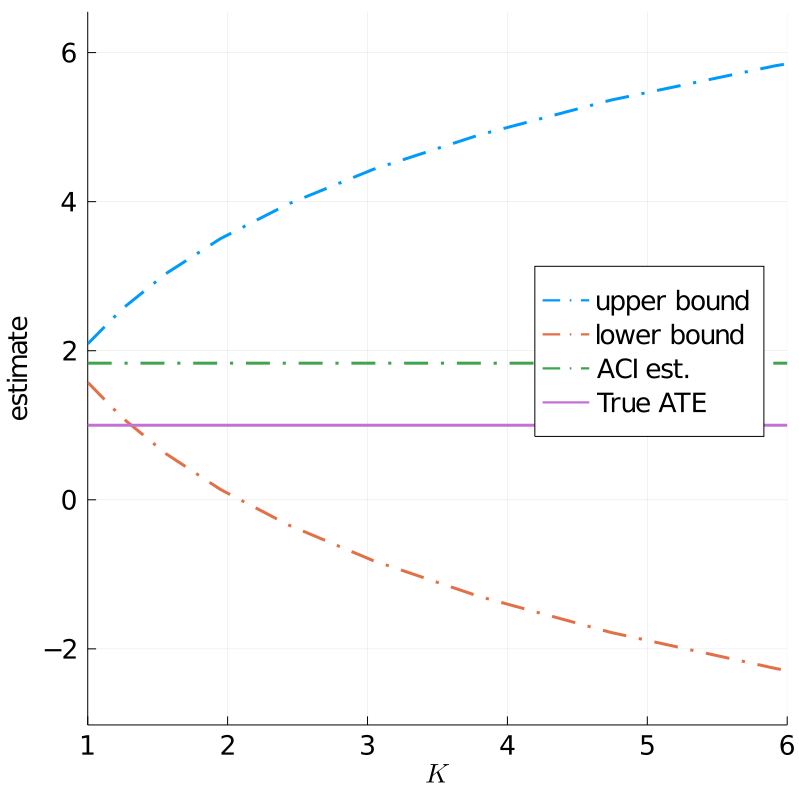
\includegraphics[width=0.6\textwidth]{../code/fig1.png}
        % \caption{}
        \label{fig:fig1}
    \end{figure}
\end{frame}

\begin{frame}{Histogram of Simulated Bounds: $n = 2000, K(H) = 1.2$}
    \begin{figure}
        \centering
        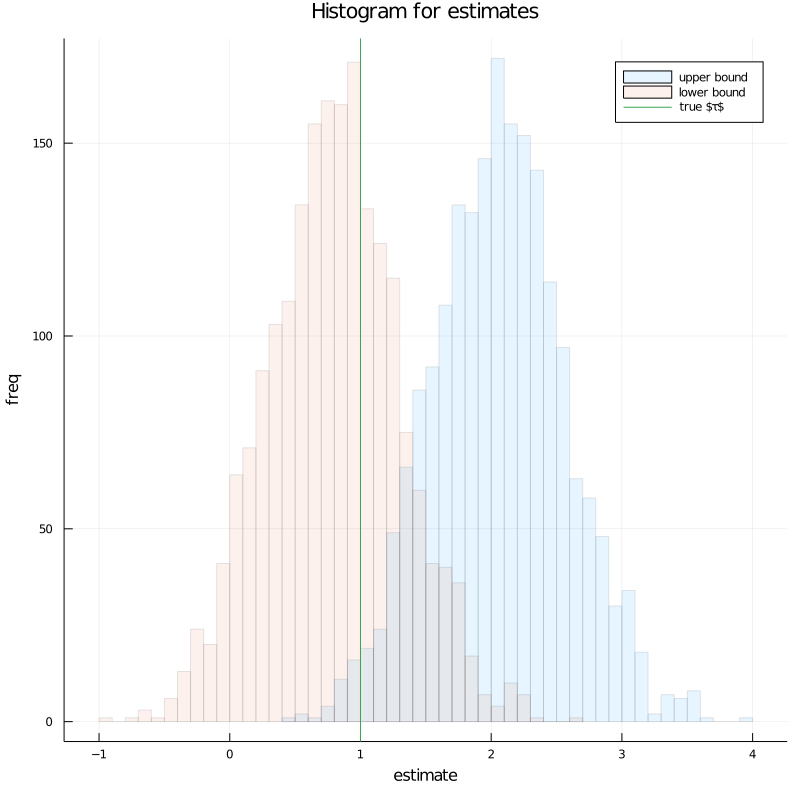
\includegraphics[width = 0.7 \textwidth]{../code/fig2.png}
        % \caption{}
        \label{fig:fig2}
    \end{figure}
\end{frame}

\begin{frame}

    \begin{table}
        \begin{adjustbox}{width=\textwidth, totalheight=\textheight-2\baselineskip,keepaspectratio}
        \centering
        \begin{threeparttable}
            \caption{Monte Carlo Results: $B = 2000, \tau = 1, K = H = 1.2$}
                \begin{tabular}{|c|c|c|c|c|c|c|c|}
                \hline $\mathrm{n}$ & $\widehat{\tau}^{-}$ & $\widehat{\sigma}^{-}$ & \text {Std. dev. of } $\widehat{\tau}^{-}$ & $\widehat{\tau}^{+}$ & $\widehat{\sigma}^{+}$ & \text {Std. dev. of } $\widehat{\tau}^{+}$ & \text {Coverage } \\
                \hline 500 & 0.704 & 0.745 & 0.746 & 1.985 & 0.744 & 0.748 & 0.989 \\
                1000 & 0.730 & 0.526 & 0.518 & 1.993 & 0.525 & 0.516 & 0.992 \\
                2000 & 0.749 & 0.370  & 0.376 & 2.000 & 0.371 & 0.375 & 0.996 \\
                \hline
                \end{tabular}
                \label{tab:tab2}
            \begin{tablenotes}
              \small
              \item Coverage statistics from $B = 2000$ simulations generated from the model specified above. The true ATE in the simulation is $\tau = 1$, and unobserved confounding is chosen such that simulation satisfies $K = H = 1.2$. Std. dev. of $\tau^-$ refers to standard deviation between simulation runs (likewise for $\tau^+$). Coverage is for estimated 95\% confidence intervals $(\hat{\tau}^- - 1.96 \hat{\sigma}^-, \hat{\tau}^+ + 1.96 \hat{\sigma}^+)$. These are conservative because the true model cannot simultaneously be upward biased and downward biased.
            \end{tablenotes}
          \end{threeparttable}
\end{adjustbox} 
  \end{table}

\end{frame}

\begin{frame}
    \begin{table}
        \begin{adjustbox}{width=0.8\textwidth, totalheight=\textheight-2\baselineskip,keepaspectratio}
        \centering
        \begin{threeparttable}
            \caption{Monte Carlo Results: $B = 2000, \tau = 1, K = H = 1$}
                \begin{tabular}{| c | c | c | c | c | c |}
                \hline $\mathrm{n}$ & $\widehat{\tau}^{-}(\widehat{\tau}^{+})$ & $\widehat{\sigma}^{-}(\widehat{\sigma}^{+})$ & \text {Std. dev. of } $\widehat{\tau}^{-}(\widehat{\tau}^{+})$ & \text {Coverage } \\
                \hline 500 & 1.038 & 0.727 & 0.732  & 0.955 \\
                1000 & 1.039 & 0.511 & 0.508  & 0.945 \\
                2000 & 1.029 & 0.362 & 0.352 & 0.947 \\
                \hline
                \end{tabular}
                \label{tab:tab1}
            \begin{tablenotes}
              \small
              \item Coverage statistics from $B = 2000$ simulations generated from the model specified above. The true ATE in the simulation is $\tau = 1$, and unobserved confounding is chosen such that simulation satisfies $K = H = 1$. Std. dev. of $\tau^-$ refers to standard deviation between simulation runs (likewise for $\tau^+$. Coverage is for estimated 95\% confidence intervals $(\hat{\tau}^- - 1.96 \hat{\sigma}^-, \hat{\tau}^+ + 1.96 \hat{\sigma}^+)$. In this case, $\tau^-$ and $\tau^+$ coincide. 
            \end{tablenotes}
          \end{threeparttable}
\end{adjustbox}
  \end{table}
\end{frame}

\section{Conclusion}

\begin{frame}{Conclusion}
    \begin{itemize}
        \item I propose a method that can be be used to perform sensitivity analysis for the estimation scheme in ACI (2020) which focuses on long-term treatment effects
        \item Bounds on the treatment effect based on relaxation of likelihood ratio are available, and the propagation of sensitivity is naturally incorporated
        \item Easy-to-implement estimator and inference procedure
        \item Valid but often over-conservative CI as shown by the Monte Carlo evidence
    \end{itemize}    
\end{frame}

\section{Appendix}

\begin{frame}{Interpretation}
    \begin{lem}[Adapted from YNBDT(2018)]
            Suppose $$Y(1) \perp D \mid S(1), U.$$
            $\Gamma$ confoundedeness is equivalent as the following:
                The log odds ratio can be written as $$\log \left(\frac{P(D=1 \mid S(1) = s, U=u)}{P(D=0 \mid S(1)=s, U=u)}\right)=\kappa(s)+\log (\Gamma) b(u)$$
                where $u$ stands for the unmeasured confounding variable, $b(u)$ is some real-valued function that takes value in $[-1,1]$.
        \end{lem}
        \begin{itemize}
            \item Similar interpretation of $H$-comparability
        \end{itemize}
\end{frame}

\begin{frame}{Side Note: Sharpness}
    \begin{itemize}
        \item It is possible for a DGP to satisfy $K-$confoundedness and $H-$comparability but does not attain the bounds
        \item Marginally sharp does {\color{red} not} imply jointly sharp
        \item The confounders $U$ (for latent-unconfoundedness) and $V$ (for sample comparability) can be correlated, and the previous analysis need to be done after orthogonalization of these two confounders (ongoing work)
    \end{itemize}
\end{frame}

\end{document}